\documentclass[a4paper]{ctexart}

%插图
\usepackage{graphicx}
%盒子
\usepackage[most]{tcolorbox}
%设置脚注
\usepackage[noadjust]{marginnote}
\renewcommand*{\raggedleftmarginnote}{}
\renewcommand*{\raggedrightmarginnote}{}
\usepackage[marginal]{footmisc}
%特殊符号及数学符号
\usepackage{pifont}
\usepackage{amssymb,amsmath}
\usepackage{breqn}
\usepackage{pxfonts}

%设置列表环境的标号以及引用,如需设置多层级请自行参阅宏包使用手册
\usepackage{enumitem}
\setlist[enumerate,1]{label = (\arabic*),
	ref   = (\arabic*)}
%设置页面尺寸
\usepackage[left=2cm,right=2cm,top=1.5cm,bottom=1.5cm]{geometry}
%页眉页脚
\usepackage{fancyhdr} 
\pagestyle{plain}
%定义脚注
\makeatletter
\renewcommand\thefootnote{\myfootnotestyle{\arabic{footnote}}}
\def\@makefnmark{\hbox{\textsuperscript{\@thefnmark}}}
\newcommand\myfootnotestyle[1]{\ifcase#1 \or \ding{182}\or \ding{183}\or
	\ding{184}\or \ding{185}\or \ding{186}\or \ding{187}%
	\or \ding{188}\or \ding{189}\or \ding{190}\or \ding{191}\else *\fi\relax}
\makeatother

%%图文混排
\usepackage{picinpar}
%无法推导出符号定义
\newcommand{\notimplies}{%
	\mathrel{{\ooalign{\hidewidth$\not\phantom{=}$\hidewidth\cr$\implies$}}}}

%TikZ设置
\usepackage{tikz}
\usepackage[tikz]{bclogo}
\usepackage{tikzpagenodes}
\tcbuselibrary{skins}

%超链接
\usepackage[hidelinks]{hyperref}

%定义颜色
\usepackage{xcolor}
\definecolor{thinkcolor}{RGB}{227,196,144}
\definecolor{thinkcolor2}{RGB}{172,128,75}
\definecolor{observecolor}{RGB}{153,201,227}
\definecolor{explorecolor}{RGB}{178,217,200}
\definecolor{textcolor1}{RGB}{77,174,234}

\tcbset{
    common/.style={
		enhanced,
		arc=0mm,
		fonttitle=\large\bfseries,
		coltitle=black,
		attach boxed title to top left={xshift=0mm,
										yshift=-0.50mm},
		boxed title style={
			skin=enhancedfirst jigsaw,
			size=small,
			arc=5mm,
			bottom=0mm,
			left=8mm,
			right=26mm,
			top=1mm},
			boxrule=0pt,
			frame hidden},
    thinkstyle/.style={
		common,
		colbacktitle=thinkcolor,
		colframe=thinkcolor,
		colback=thinkcolor!40,
		borderline north={4pt}{0pt}{thinkcolor}},
	observestyle/.style={
		common,
		colbacktitle=observecolor,
		colframe=observecolor,
		colback=observecolor!40,
		borderline north={4pt}{0pt}{observecolor}},
	explorestyle/.style={
		common,
		colbacktitle=explorecolor,
		colframe=explorecolor,
		colback=explorecolor!40,
	borderline north={4pt}{0pt}{explorecolor}},
	before upper={\parindent1em}		%设置段首缩进
}	
%颜色
\newtcolorbox{think0}{thinkstyle,title= \raisebox{-0.1cm} { \hspace{-0.35cm} 
\includegraphics{logo1}} \  \raisebox{0.1cm} { \color{olive} \zihao{4} 思 \ 考} } 
\newtcolorbox{think}{thinkstyle,title=     \raisebox{-0.2cm}{\bcquestion }   \color{olive} \zihao{4} 思 \ 考 }  
\newtcolorbox{observe0}{observestyle,title= \raisebox{-0.15cm}{\hspace{-0.2cm} 
\includegraphics{logo2}} \  \color{yellow}  \zihao{4} 观\ 察}
\newtcolorbox{observe}{observestyle,title=   \raisebox{-0.2cm}{\bcfleur}  \color{yellow}  \zihao{4}  \ 观 \ 察}
\newtcolorbox{explore0}{explorestyle,title = \raisebox{-0.15cm} {
\includegraphics{logo3} \  \raisebox{0.15cm}{
	\color{teal} \zihao{4}	 探\ 索}}}
\newtcolorbox{explore}{explorestyle,title =    \raisebox{-0.2cm}{ \bclampe}  \ \color{teal}  \zihao{4} 探 \ 索}

\newtcolorbox{custom}[2][gray]{
	common,
	title=#2,
	colbacktitle=#1,
	colframe=#1,
	colback=#1!40,
	borderline north={4pt}{0pt}{#1}}


\begin{document}
	
\begin{think}
	下列``若 $p$ ,则 $q$ '' 形式的命题中,哪些是真命题?哪些是假命题?
	\begin{enumerate}
		\item 若平行四边形对角线相互垂直,则这个平行四边形是菱形;	\label{item1-1}
		\item 若两个三角形周长相等,则这两个三角形全等;							\label{item1-2}
		\item 若 $x^2 - 4x + 3 =  0$,则 $x=1$;													\label{item1-3}
		\item 若平面内两条直线 $a$ 和 $b$ 均垂直于直线 $l$ ,则 $a  \parallel b$; \label{item1-4}
	\end{enumerate}
\end{think}
  在命题 \ref{item1-1} \ref{item1-4} 中,由条件 $p$ 通过推理可以得出结论 $q$,所以它们是真命题,在命题 \ref{item1-2} \ref{item1-3} 中,
  由条件 $p$  不能得出结论 $q$ ,所以它们是假命题.
  
  一般地,若 $p$,则 $q$ 为真命题,是指由 $p$ 通过推理得出 $q$。 这时,我们就说,由 $p$ 可以推出 $q$,记作
  	\[  p  \implies q,
  	\]
	并且说,$p$ 是 $q$ 的 \textcolor{textcolor1}{充分条件} (sufficient condition),$q$ 是 $p$ 的 \textcolor{textcolor1}{必要条件} \footnote{测试一下脚注} (necessary condition).
	
	如果 `` 若 $p$,则 $q$ '' 为假命题,那么由条件 $p$ 不能推出结论 $q$,记
	作$p \notimplies q$ ,此时,我们就说 $p$ 不是 $q$ 的充分条件,$q$ 不是 $p$ 的必要条件
	
	上述命题 \ref{item1-1} \ref{item1-4} 中的 $p$ 是  $q$ 的 充分条件, $q$ 是 $p$ 的必要条件.
	
\begin{explore} 
	通过上面的学习,你能给出``四边形是平行四边形''的充要条件吗?
\end{explore}
	可以发现,``四边形的两组对角分别相等''``四边形的两组对边分别相等''``四边形的一组对边平行相等''
	和``四边形的对角线互相平分''既是``四边形是平行四边形'' 的充分条件,又是必要条件,所以它们都是
	``四边形是平行四边形''  的充要条件
	 
	 另外,我们再来看看平行四边形的定义:
	 \begin{center}
	 	两组对边分别平行的四边形叫做平行四边形,
	 \end{center} 
	它表明``四边形的两组对边分别平行'' 也是 ``四边形是平行四边形''的一个充要条件.
	
\begin{observe}
 	 观察下面几个例子,类比实数之间之间的相等关系、大小关系,你能发现下面几个集合之间的关系吗?
 	 \begin{enumerate}
 	 	\item $A = \{ 1,2,3 \},B = \{1,2,3,4,5  \} ;$  \label{item3-1}
 	 	\item $C$ 为立德中学高一 (2) 班全体女生的集合,$D$ 为这个班全体学生组成的集合;  \label{item3-2}
 	 	\item $E = \{x|  x \  \text{是两条边相等的三角形 } \} $, $F =  \{x| x \text{\ 是等腰三角形}  \} $. \label{item3-3}
 	 \end{enumerate}
\end{observe}


   

  	可以发现,在 \ref{item3-1} 中, 集合 $A$ 的任何一个元素都是集合 $B$ 的元素,这时我们说集合 $A$ 包含于集合 $B$ ,或集合 $B$ 包含集合 $A$.  \ref{item3-2} 中的集合 $C$ 与 集合 $D$ 也有这种关系.
   	
   	\begin{figwindow}[1,r, \mbox{\vspace{1em} 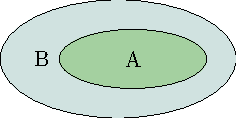
\includegraphics{picture.pdf}},{集合图}]
   		   	一般地,对于两个集合 $A$,$B$ ,如果集合 $A$ 中任意一个元素都是集合 $B$ 中的元素,就称集合 $A$ 为集合 $B$ 的  \textcolor{textcolor1}{子集} (subset), 记作 
   	\end{figwindow}

   	  \[  A \subseteq B ( \text{或} B  \supseteq A) ,
   	\]
   	读作 ``A 包含于 B'' (或 ``B 包含 A '') .

\newpage 

\begin{think0}
	下列``若 $p$ ,则 $q$ '' 形式的命题中,哪些是真命题?哪些是假命题?
	\begin{enumerate}
		\item 若平行四边形对角线相互垂直,则这个平行四边形是菱形;	\label{item1-1}
		\item 若两个三角形周长相等,则这两个三角形全等;							\label{item1-2}
		\item 若 $x^2 - 4x + 3 =  0$,则 $x=1$;													\label{item1-3}
		\item 若平面内两条直线 $a$ 和 $b$ 均垂直于直线 $l$ ,则 $a  \parallel b$; \label{item1-4}
	\end{enumerate}
\end{think0}
在命题 \ref{item1-1} \ref{item1-4} 中,由条件 $p$ 通过推理可以得出结论 $q$,所以它们是真命题,在命题 \ref{item1-2} \ref{item1-3} 中,
由条件 $p$  不能得出结论 $q$ ,所以它们是假命题.

一般地,若 $p$,则 $q$ 为真命题,是指由 $p$ 通过推理得出 $q$。 这时,我们就说,由 $p$ 可以推出 $q$,记作
\[  p  \implies q,
\]
并且说,$p$ 是 $q$ 的 \textcolor{textcolor1}{充分条件} (sufficient condition),$q$ 是 $p$ 的 \textcolor{textcolor1}{必要条件} \footnote{测试一下脚注} (necessary condition).

如果 `` 若 $p$,则 $q$ '' 为假命题,那么由条件 $p$ 不能推出结论 $q$,记
作$p \notimplies q$ ,此时,我们就说 $p$ 不是 $q$ 的充分条件,$q$ 不是 $p$ 的必要条件

上述命题 \ref{item1-1} \ref{item1-4} 中的 $p$ 是  $q$ 的 充分条件, $q$ 是 $p$ 的必要条件.

\begin{explore0} 
	通过上面的学习,你能给出``四边形是平行四边形''的充要条件吗?
\end{explore0}
可以发现,``四边形的两组对角分别相等''``四边形的两组对边分别相等''``四边形的一组对边平行相等''
和``四边形的对角线互相平分''既是``四边形是平行四边形'' 的充分条件,又是必要条件,所以它们都是
``四边形是平行四边形''  的充要条件

另外,我们再来看看平行四边形的定义:
\begin{center}
	两组对边分别平行的四边形叫做平行四边形,
\end{center} 
它表明``四边形的两组对边分别平行'' 也是 ``四边形是平行四边形''的一个充要条件.

\begin{observe0}
	观察下面几个例子,类比实数之间之间的相等关系、大小关系,你能发现下面几个集合之间的关系吗?
	\begin{enumerate}
		\item $A = \{ 1,2,3 \},B = \{1,2,3,4,5  \} ;$  \label{item3-1}
		\item $C$ 为立德中学高一 (2) 班全体女生的集合,$D$ 为这个班全体学生组成的集合;  \label{item3-2}
		\item $E = \{x|  x \  \text{是两条边相等的三角形 } \} $, $F =  \{x| x \text{\ 是等腰三角形}  \} $. \label{item3-3}
	\end{enumerate}
\end{observe0}




可以发现,在 \ref{item3-1} 中, 集合 $A$ 的任何一个元素都是集合 $B$ 的元素,这时我们说集合 $A$ 包含于集合 $B$ ,或集合 $B$ 包含集合 $A$.  \ref{item3-2} 中的集合 $C$ 与 集合 $D$ 也有这种关系.

\begin{figwindow}[1,r, \mbox{\vspace{1em} 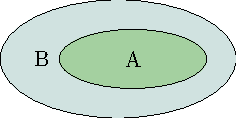
\includegraphics{picture.pdf}},{集合图}]
	一般地,对于两个集合 $A$,$B$ ,如果集合 $A$ 中任意一个元素都是集合 $B$ 中的元素,就称集合 $A$ 为集合 $B$ 的  \textcolor{textcolor1}{子集} (subset), 记作 
\end{figwindow}

\[  A \subseteq B ( \text{或} B  \supseteq A) ,
\]
读作 ``A 包含于 B'' (或 ``B 包含 A '') .








\end{document}